\documentclass[answers,12pt]{exam}

\setlength{\parindent}{0cm} % global indent value

\usepackage{graphicx}
\usepackage{mhchem}
\usepackage{wrapfig}

\pagestyle{headandfoot}
\runningheadrule
\firstpageheader{name:\fillin[][4cm]}{period:\fillin[][1cm]}{Unit 2: Combustion}
\runningheader{Unit 2: Combustion}
{Class Notes}
{Page \thepage\ of \numpages}
\firstpagefooter{}{}{}
\runningfooter{PACS}{Mr. Maxwell}{page \thepage\ of \numpages}


\begin{document}

\section{Lesson 2.1 Computing the Energy in Food}

\begin{itemize}
    \item The modern metric unit of energy is the \fillin[joule]. 
    \item An older unit of energy is the \fillin[calorie].
    \item To convert use: \fillin[1] calorie = \fillin[4.2] joules
    \item A food calorie = 1000 energy calories = 1 kilocalorie = 1 kcal
\end{itemize}
    

\begin{wrapfigure}{r}{0.5\textwidth} %this figure will be at the right
    \centering
    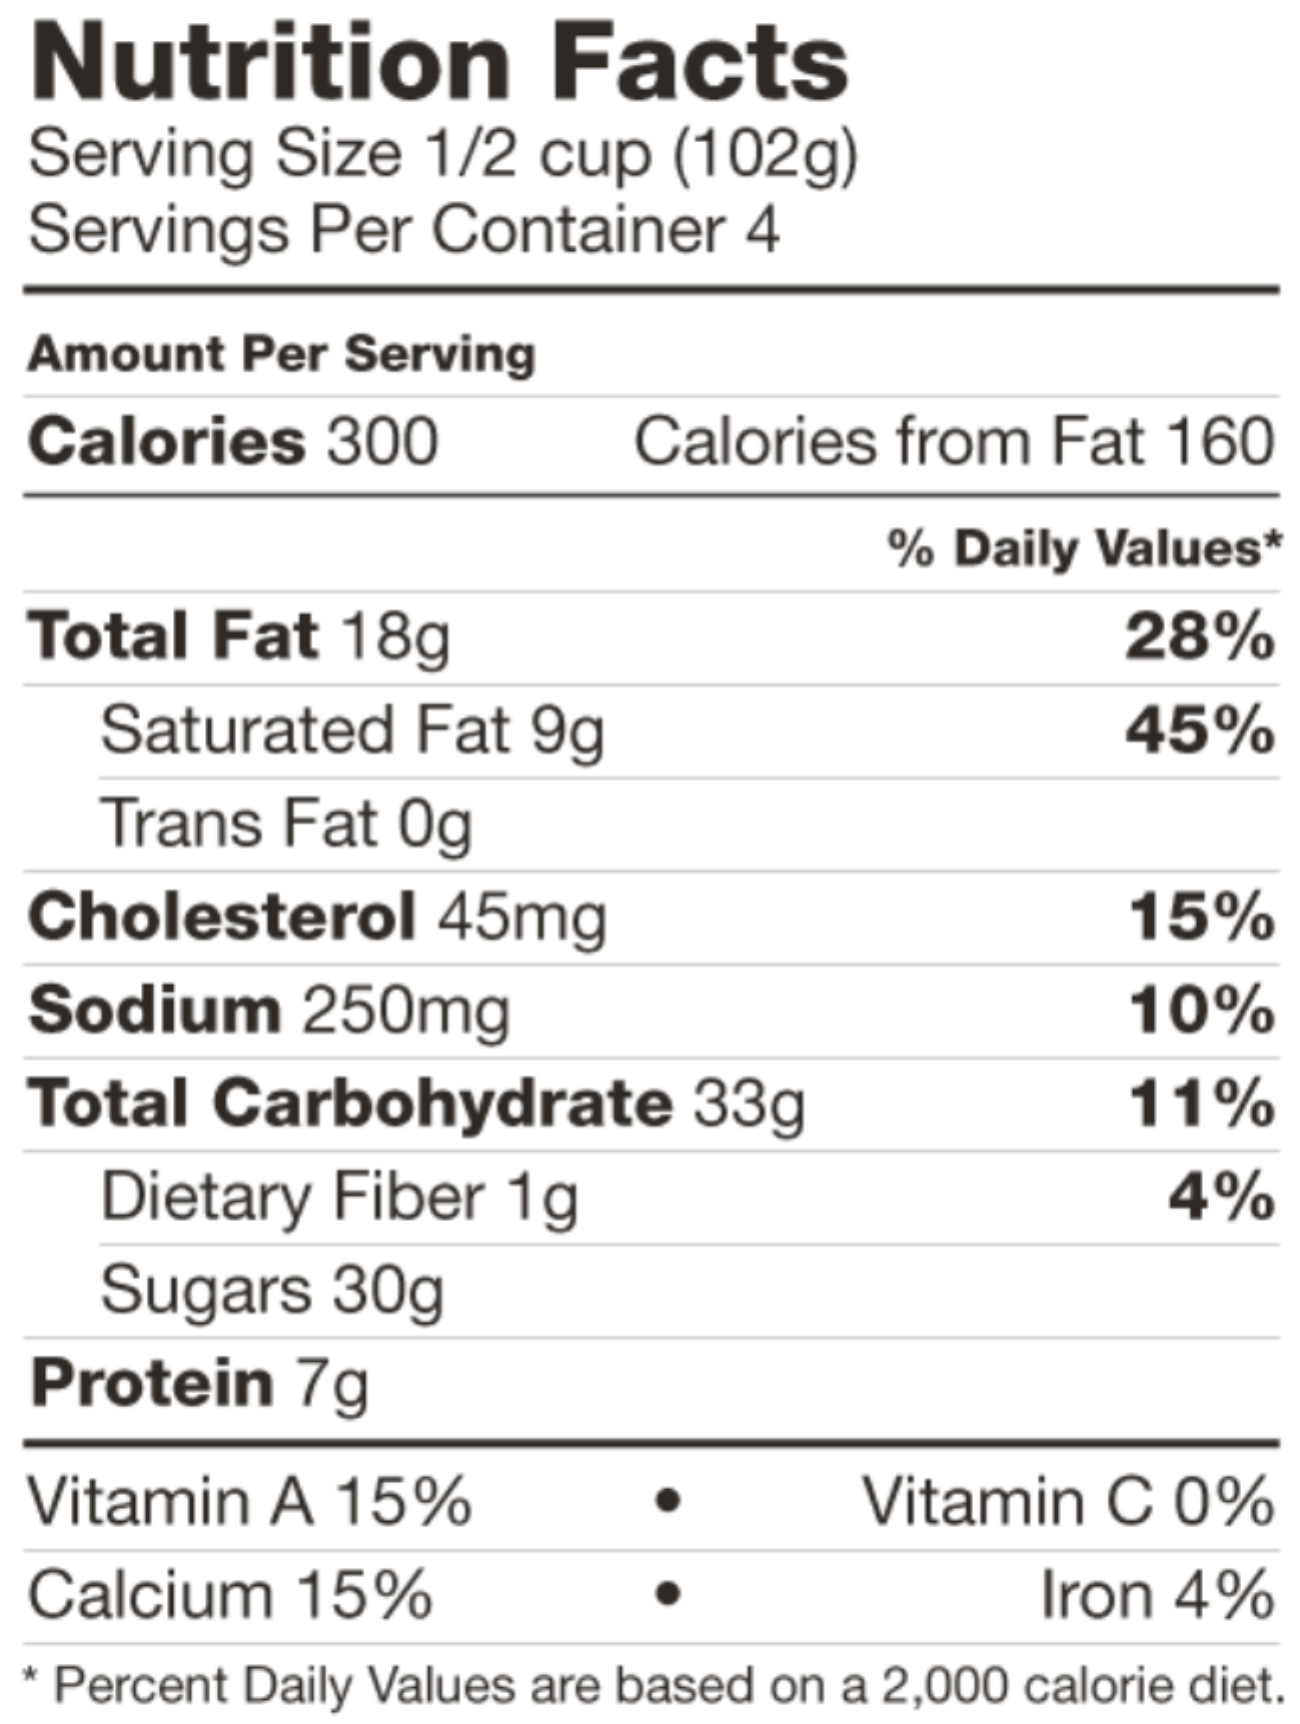
\includegraphics[width=0.35\textwidth]{food_label.png}
\end{wrapfigure}


Find the \textbf{grams per serving} \\ 

Find the food \textbf{calories per serving} on the label - remember that these are actually kcal of energy. \\

Compute the kcal per gram:

$$ calories \; per \; serving = \fillin[300] kcal $$
$$ grams \; per \; serving = \fillin[102] g $$

$$ kcal/g = \frac{calories \; per \; serving}{grams \; per \; serving} = \fillin[2.9] kcal/g  $$

\vspace{1cm}




    
    
\end{document}